% This is samplepaper.tex, a sample chapter demonstrating the
% LLNCS macro package for Springer Computer Science proceedings;
% Version 2.21 of 2022/01/12
%
\documentclass[runningheads]{llncs}
%
\usepackage[T1]{fontenc}
% T1 fonts will be used to generate the final print and online PDFs,
% so please use T1 fonts in your manuscript whenever possible.
% Other font encondings may result in incorrect characters.
%
\usepackage{graphicx}
\usepackage{enumitem}
\setlist[enumerate]{label*=\arabic*.}
\usepackage{adjustbox,lipsum}
\usepackage{array}
\usepackage{pgfplots}
\usepackage{tikzscale}
% Used for displaying a sample figure. If possible, figure files should
% be included in EPS format.
%
% If you use the hyperref package, please uncomment the following two lines
% to display URLs in blue roman font according to Springer's eBook style:
%\usepackage{color}
%\renewcommand\UrlFont{\color{blue}\rmfamily}
%\urlstyle{rm}
%

%\usepackage[sectionbib,numbers,sort&compress]{natbib}
%\bibliographystyle{splncs04nat}

\begin{document}
%
\title{Usage of process mining for security in Process-Aware Information Systems}
%
\titlerunning{Process Mining for security in PAIS}
% If the paper title is too long for the running head, you can set
% an abbreviated paper title here
%
\author{Marlon Müller\inst{1}}
%
\authorrunning{M. Müller}
% First names are abbreviated in the running head.
% If there are more than two authors, 'et al.' is used.
%
\institute{
    Technical University of Munich, Munich, Germany\\
    \email{marlonbenedikt.mueller@tum.de}}
%
\maketitle              % typeset the header of the contribution
%
\begin{abstract}
    Security in Process-Aware Information System (PAIS) is critical for almost every organisation and company, as a lack of security measures leads to vulnerabilities that can, if abused, cause severe fincancial damage.
    The survey~\cite{Leitner2014273} by Leitner and Rinderle-Ma from 2013 analysed in a systematic literature review the researched security controls in PAIS\@. The authors identified that the usage
    of Process Mining may be an emerging topic, so this paper provides a systematic literature review to analyze the advances in Process Mining research for security in PAIS and clusters the results
    by the security goals that are protected as well as the Process Mining applications and concpets that can be used for security in PAIS\@.

    \keywords{Process Mining \and Security \and Process-Aware Information Systems \and Systematic literature review.}
\end{abstract}
%
%
%
\section{Introduction}\label{Introduction}
In 2018 76\% of businesses in Germany saw a significant risk for their business processes coming from cyberattacks on their information systems~\cite{Bsi} and in a report by the
Federal Bureau of Investigation from 2023 companies in the
United States reported total damages of 37.5 billion US-Dollars due to cybercrime~\cite{fbi}. This shows the need for companies to protect their business processes from cyberattacks.\\
Therefore over the last years the research in security for Process-Aware Information Systems (PAIS) has increased and has produced a vast amount of research papers. The survey~\cite{Leitner2014273}
conducted a systematic literature review on security in PAIS and identified Process-Mining as an emerging technology that can be used to improve security in PAIS and predicted that
the usage of Process Mining for security purposes in PAIS will be a focus of future research.\\
In 2018, already 65\% of German businesses investigated log-files to identify security incidents based on the suspicion of a security incident and 33\% use log-files to systematically
identify security incidents without concrete suspicions~\cite{Bsi}.\\
Therefore Process Mining has the potential to be further enhanced to be used for security in Process-Aware Information Systems and was further researched in the last years. This paper
aims to update the survey by Leitner and Rinderle-Ma~\cite{Leitner2014273} in the field of Process Mining and to provide an overview over the recent advances in the usage of Process Mining for security purposes in PAIS since 2012. For this goal we will conduct a systematic literature
review to outline the possible applications of Process Mining for security in PAIS.\\
\\
To approach this goal the following research questions were targeted:
\begin{enumerate}
    \item How does Process Mining contribute to security in PAIS\@?
    \item Have the research challenges defined in~\cite{Leitner2014273} been addressed by recent research?
\end{enumerate}

In Section~\ref{Fundamentals} we will first provide some defintions and explanaitions over the terms used in this paper.
Section~\ref{Related} evaluates related works in this field and how this paper adds further contribution to current research.
Section~\ref{Methodology} outlines the different steps of the literature review consisting of literature search, literature selection, data extraction and the classification of security goals and security concepts.
The results of the literature review are described in Section~\ref{Results} and in Section~\ref{Conclusion} the results are discussed and the paper is concluded.

\section{Fundamentals}\label{Fundamentals}
Below definitons for the most relevant terms in this paper are provided.
\subsection{Process Mining}\label{Process Mining}
The main idea of Process Mining is to extract knowledge from event logs generated by existing information systems. Because event logs are often stored in an unstructured format, Process Mining uses Data Science approaches to
extract the desired information in an format that can easily be analyzed by humans.\cite{vanderAalst2016} Because Process Mining uses Data Science approaches, such as data mining or machine learning, it can be seen as the bridge between Data Science and Process Science.\\
Process Mining can be used for
\begin{itemize}
    \item Process Discovery: The automatic generation of a process model based on the information extracted from an event log.
    \item Conformance Checking: Compare the event log of a process execution with the formal process model of that process to detect deviations.
    \item Enhancement: Usage of the actual process execution extracted from the event log to extend or improve an existing process model.
\end{itemize}

\subsection{Information Security}\label{Security}
Security in Information Systems (also called Information Security) is defined by the International Organization for Standardization (ISO) as the protection of
Confidentiality, Integrity and Availabilty of information~\cite{ISO}. This definition is also known as the CIA-Properties, but can be extended by other security goals as defined below. In other
literature the term Information Security describes the protection of systems to enter a state that allows unauthorized access to information or resources. This means, that security involves an
unauthorized entity (the attacker). Security can differentiated from safety by the fact that safety describes the ability of a system to be prone to software or hardware failures from within
the system itself without the influence of an attacker.\cite{Eckert}\\
\subsubsection{Security Goals}\label{goals_def}
Later in this paper the results will be clustered according to the security goals that are protected by the applications proposed by the reviewed papers (Section~\ref{Methodology} and~\ref{goals}).
The clusters are chosen based on the security goals as described by Eckert in~\cite{Eckert}. While the CIA-Properties (Confidentiality, Integrity, Availabilty) are commonly agreed on as the
primary security goals the other security goals (especially Privacy and Accountability) are acknowledged as valid security goals but their relevance to different use cases is discussed and
not commonly agreed on. %Hier evtl andere Literatur noch nennen.
Nonetheless this six security to goals according to~\cite{Eckert} are chosen because clustering only by the CIA-Properties would not reflect the whole bandwith of security research in Process Mining
for PAIS while still allowing clear distinctions between them. The following definitions of the different security goals are taken from~\cite{Eckert}.
\paragraph{Confidentiality} Confidentiality to protect information from being disclosed to unauthorized entities. This includes the encryption of data as well as models to restrict the flow of
information according to an organisations policies.
\paragraph{Integrity} A system is considered to have integrity if it provides protection against unauthorized and unnoticed manipulation of data or processes. To guarantee integrity
Access Control mechanisms are used to ensure that only authorized entities with the proper Access Rights can modify data or processes under certain constraints (e.g.\ limit the amount of money
a user can withdraw from an account). In systems where manipulations can not be avoided (e.g.\ in network communication) cryptographic hashing should be used to detect manipulations and
avoid further damages.
\paragraph{Availabilty} Availability is the property of a system to be accessible and usable by autorized entities without unauthorized delays or restrictions. Delays that are a result of the
normal operation of a system (e.g.\ concurrency over shared resources) are considered as authorized delays and therefore do not violate the property of availability.
\paragraph{Accountability} The property of accountability (sometimes referred to as non-repudiation) is to ensure that an entity can not deny the actions it has taken. Accountability is
important for Electronic Commerce to be able to prove in lawsuit that a contract has been signed by a certain entity or that a contract has been fulfilled.
\paragraph{Privacy} The ability of individuals to control the collection, use and disclosure of their personal information is called Privacy and obliges organisations to protect the data of
identified or identifiable individuals. Privacy is considered a human right~\cite{EU} and is therfore often regulated by laws like the General Data Protection Regulation (GDPR) in the European Union.
\paragraph{Authenticity} Authenticity is the valiation of the identity of an acting entity using unique identifiers or characteristics, such as cryptographic keys or biometric data.
The act of verifying the identity of an entity is called authentication, that happens typically using user accounts with a distinct username and a secret password and/or biometric factors.
The data that is used to verify the identity (e.g.\ the password) is called credentials to provide an abstraction of the concrete authentication method used.
\subsection{Process-Aware Information Systems}\label{PAIS}
The term Process-Aware Information Systems is definded by Dumas et al.~\cite{Dumas20051} by combining the definitions of Information Systems (as PAIS are a special kind of Information Systems)
and business processes. Their understanding of a business process is a ``way for an organizational entity to organize work and resources (\ldots) to accomplish its aims''. On that foundation
PAIS are defined as ``a software system that manages and executes operational processes involving people, applications, and/or information sources on the basis of process models''.
Additionally to the formal defintion they marked that these process models are often represented using visual languages, like Petri-Net notations.\\
The main difference between a PAIS and a task-driven Information System (e.g.\ text editor or e-mail client) is described as the fact that task-driven applications are unaware of the process
they are used in and therefore can neither support nor restrict the user in the process execution. By this differentiation PAIS are also defined as systems that support prcesses Instead of only isolated activities.\cite{vanderAalst2016}
\section{Related Work}\label{Related}
In this section the survey by Leitner and Rinderle-Ma~\cite{Leitner2014273}, that this paper aims to update, is briefly summarized and other related works are presented and explained how
this paper adds further contribution to the research in Process Mining for security in PAIS.\\
\subsection{Survey by Leitner and Rinderle-Ma from 2013}\label{basepaper}
The main objective of this paper is to update the systematic literature review conducted in~\cite{Leitner2014273} regarding the Process Mining security control and to provide an overview over the recent advances
in the usage of Process Mining for security purposes in PAIS until 2012.
\subsubsection{Summary of the survey}\label{Summary}
In that survey the authors identified Process Mining as an emerging technology and gave a brief overview
over the security related research regarding Process Mining in PAIS\@. The authors assigned Process Mining to the action type Detection and placed it in the Change phase of the
process lifecycle.\\
In this survey the authors assigned Process Mining the action type Detection and placed it in the Change phase of the process lifecycle. They identified that the main usage of
Process Mining for security purposes in PAIS is to examine the conformance of the process model with the actual process execution that could be derived from the event logs.
The derived model from the event logs can be used to detect inconsitencies and anomalious behaviour that could be an indicator for security incidents like fraud or intrusions.
Another use case the authors identified is to use event logs to validate the conformity of the process execution with the security policies of the company, like
Role-Based Access Control (RBAC) models or data flow
policies. It was concluded, that Process Mining can be used to capture relevant information on data, ressources and task execution to find or address security issues and compliance
violations and their root causes.\\
\subsubsection{Research Challenges identified}\label{Challenges}
For security in PAIS in general (and not only regarding Process Mining) the authors identified the following research challenges:
\begin{enumerate}
    \item Agreement on Terminology and Controls
    \item Consistency with Related Fields and Concepts
    \item Measurement
    \item Testing
    \item Evaluation
    \item Detection Controls
    \item Reaction Controls
    \item Human Orientation
\end{enumerate}
\paragraph{Agreement on Terminology and Controls} The authors identified that the terminology used in the field of security in PAIS is not consistent and in some research no
defintion of security or the protected security goals are provided.
\paragraph{Consistency with Related Fields and Concepts} Even though research in security in PAIS is an interdisciplinary field, it was identified that except for the NIST standard for
RBAC no standards or recoommendations are considered in the research.
\paragraph{Measurement} The authors could not identify any methods or metrics are used to evaluate the effectiveness of the security controls in PAIS, while in other security areas
well developed standards, e.g.\ the ISO/IEC 27004 standard, exist.
\paragraph{Testing} Most of the security concepts in PAIS research are theoretical models and no method to test these models is provided.
\paragraph{Evaluation} In the examined research the evaluation of the security in PAIS centers on post-ex evaluation using Process Mining techniques and the authors stated that It
should be considered how to evaluate the security in PAIS at design or run time.
\paragraph{Detection Controls} Invastigations of possible security incidents does not happen at run time but the authors identified that it could be benficial to detect anomalies
at run time to then be able to react to them.
\paragraph{Reaction Controls} So far, reaction controls are focused on failure handling such as exception handling or process recovery. The authors identified that it could be beneficial
to react to identified security problems at design time.
\paragraph{Human Orientation} Human factors are not considered in the research instead it only focuses on the technological aspects of security in PAIS\@. The authors stressed that
humans are an important factor in business processes and that they also could be a security risk if they are psychologically manipulated during Social Engineering attacks.
\subsection{Other Systematic Literature Reviews}\label{Other}
The surveys~\cite{Kelemen_2018} and~\cite{Silalahi20221} also conducted systematic literature reviews on the usage of Process Mining in security applications. The systematic literature review
by Kelemen focused on the topics covered and the main challenges in Process Mining in the security domain~\cite{Kelemen_2018}, while the survey by Silalahi et al.\ identified the datasets,
methods, tools and frameworks used in Process Mining research~\cite{Silalahi20221}. Both surveys gave a broad overview over the research in Process Mining for security applications but did not
focus on security in PAIS\@.\\
This paper provides further contribution as it gives a more in depth analysis over the usage of Process Mining for security in PAIS\@. It also gives a unique classification of the research by
identifying the security goals that are protected. As this paper narrowing down the specific research field it takes a broader and more up-to-date time frame into consideration as~\cite{Silalahi20221} only reviewed
papers between 2017 and 2021 and~\cite{Kelemen_2018} reviewed papers between 2000 and 2016.
\section{Methodology}\label{Methodology}
The systematic literature review conducted in this paper follows the guidelines outlined in~\cite{BRERETON2007571} and is also based on the methodology used in the systematic literature review by Leitner and Rinderle-Ma~\cite{Leitner2014273}.
At first a clear definition of the research questions is given before in the second step an extensive literature search is conducted. The resulting data based on the literature search is then analysed and synthesized to answer the research questions by clustering
the papers into different categories.\\
\subsection{Research identification}\label{Identification}
This paper aims to update the survey by Leitner and Rinderle-Ma~\cite{Leitner2014273} in the field of Process Mining and security in PAIS  and therefore to examine and evaluate the advances of security research using Process Mining in PAIS since 2012.
To approach this goal we redefine the research questions formulated in Section~\ref{Introduction}:
\begin{enumerate}
    \item What is the contribution of security research using Process Mining in PAIS\@?
          \begin{enumerate}
              \item What security goals are protected by the applications proposed by the reviewed papers?
              \item What Process Mining applications and concepts are used for security in PAIS\@?
          \end{enumerate}
    \item How where the research challenges defined in~\cite{Leitner2014273} been addressed by recent research?
\end{enumerate}
The first research question is investigates the contribution of recent research in the field of Process Mining for security in PAIS and is divided into two subquestions to give a more detailed and holistic insight into the research field.
The subquestion 1.1 synthesizes the results into a classification of the security goals, as defined in Section~\ref{goals_def}, that are protected by the applications and methods proposed by the reviewed papers.
The analysis of the Process Mining applications and concepts used for security in PAIS is done in subquestion 1.2.\\
To analyze how the reviewed papers contributed and addressed the research challenges presented in~\cite{Leitner2014273} and summarized in Section~\ref{Challenges} in the second research question it is analysed what papers addressed these challenges
and how they contributed to the solution of these challenges.
\subsection{Literature Search}\label{Search}
\begin{table}[h!]
    \centering
    \caption{Inclusion and Exclusion Criteria for the Literature Search and Selection}
    \begin{tabular}{ | m{1cm} | m{11cm} | }
        \hline
        Inc 1 & Search string: („process mining“ | „data mining“) \& („security“ | „constraints“ | „access control“ | „authorization“) \& („process aware“ | „workflow“ | „business process“) \\
        \hline
        Exc 1 & The paper was published before 2013                                                                                                                                           \\
        \hline
        Exc 2 & The paper is not written in English                                                                                                                                           \\
        \hline
        Exc 3 & Title, keywords and abstract do not indicate relevance for Security, Process Mining and PAIS                                                                                  \\
        \hline
        Exc 4 & Content is not related to the usage of Process Mining to enhance security in PAIS                                                                                             \\
        \hline
        Inc 2 & Extend results by relevant papers from the references of the included papers                                                                                                  \\
        \hline
    \end{tabular}
    \label{criteria}
\end{table}
To identitfy the relevant papers for the literature review a manual search was conducted using the IEEE Xplore and Scopus databases (retrieving date: June, 17th 2024). In the literature search the search string of inclusion criteria 1 from

Table~\ref{criteria} was used with the exclusion criteria 1 and 2 applied. Those databases were chosen because they are known for their high quality of scientific papers and their relevance to the field of Computer Science. In total 261 papers were found in the search.
\subsection{Literature Selection}\label{Selection}
\begin{table}[h!]
    \centering
    \caption{Number of papers after each step of the Literature Selection}
    \begin{tabular}{ |l|l|l|}
        \hline
        \textbf{Step No.} & \textbf{Applied Criteria} & \textbf{Number of potentially rlevant Papers} \\
        \hline
        \hline
        1                 & Inc 1, Exc 1 - 2          & 261                                           \\
        \hline
        2                 & Exc 3                     & 38                                            \\
        \hline
        3                 & Exc 4                     & 15                                            \\
        \hline
        4                 & Inc 2                     & 17                                            \\
        \hline
    \end{tabular}
    \label{selection}
\end{table}
The results of the literature search were then filtered to reduce the amount of papers to the relevant literature for the topic of this review. The publications were filtered according to the scheme in Table~\ref{selection} using the inclusion and exclusion criteria
from Table~\ref{criteria}. The first step of the selection by excluding papers published before 2013 and publications not written in English was already executed during the literature search phase.
In the second step of the literature review the title, keywords and abstract of the papers were reviewed to exclude papers that did not indicate to be relevant for all three topics of Process Mining, Security \textit{and} PAIS. Because security is a broad field not all
relevant papers used the term security in their title or keywords but instead used related terms like constraints, access control or authorization. This explains the inclusion of these terms in the search strings and why it was necessary to review the abstracts in
the second step. Because the search string was designed to result in a broad range of papers about 230 irrelevant papers were excluded during step 2, resulting in 38 remaining papers.\\
A detailed filtering by the content of the publications was done in the third step. If the content did not relate to the usage of Process Mining to enhance security in PAIS the paper was excluded. In this step the main challenge was to exclude papers that were
related to Process Mining, security and PAIS but proposed methods that can make existing Process Mining applications more secure (e.g.\ by proposing secure transfer of event logs between organisations) but did not use Process Mining to enhance security in PAIS. After this step 15 papers
remained for the data selection.\\
In the last step the references of the included papers were reviewed to find further relevant papers that might have been missed in the initial search caused by the design of the search string or because they are not indexed in the databases used for the search.
The papers that were referenced by already included papers were then reviewed if they met the exclusion criteria used for the results of the initial search. In this step two additional papers were found that were referenced in~\cite{Silalahi20221}, resulting in 17
papers for the data extraction.
\subsection{Data Extraction}\label{Extraction}
In the data extraxtion phase the relevant information from the publications was extracted in order to classify the publications into a meaningful and
solid strcuture allowing to answer the research questions identified in Section~\ref{Identification}. The two steps of the data extraction
are illustrated in Figure~\ref{extract_scheme}.\\
In the first step the main security concept covered by the publication was identitfied. The identification of the main security concept was based on
title, abstract and keywords of the publication as well as the introduction and conclusion sections of the publication. It was assumed, that the authors
would indicate the publications main security concept in these sections to give the reader a brief overview over the content of the paper and to gain their
interest in the publication. For the analysis of the security concepts no automated extraction tools were used, instead the information was extracted manually.
If title, abstract, keywords, introduction and conclusion indicated multiple security concepts or gave no indication of the main security concept the
publication was inspected in more detail to identify the main security concept. During the categorization in security concepts it was always attempted
to assign the publication to the most specific security concept possible. If this was not possible a broader security concept was chosen (e.g.
Anomaly Detection is a very broad concept that could also include intrusion detection as every intrusion is also an anomaly).\\
In the second step the publications were classified into the security goals that are protected by the applications and methods proposed by the reviewed papers.
A publication could be assigned to multiple security goals if the proposed method or application covered mutiple security goals. To classify the publications it was examined
if the publication mentioned the security goals somewhere in the paper. As most of the papers did not explicitly mention the security goals, a manual classification was done by reviewing
the purposes of the proposed methods and applications.\\
In a last step it was analysed how the reviewed papers addressed the research challenges identified in~\cite{Leitner2014273}, for this purpose the content of the papers, especially the
conclusion and discussion as well as the results sections, were reviewed and their contribution to one, or more, of the research challenges was investigated.
\begin{figure}
    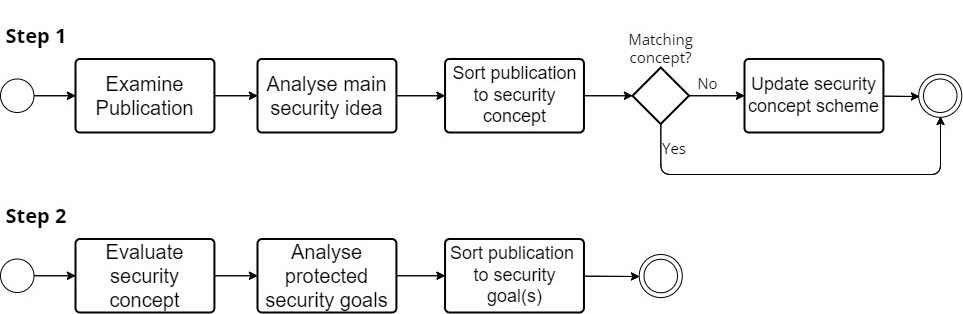
\includegraphics[width = \textwidth]{figures/extraction.jpg}
    \caption{Data Extraction Scheme}
    \label{extract_scheme}
\end{figure}
\section{Results}\label{Results}
This section will outline the results of the systematic literature review. At first, the publication years and publication sources of the selected publications is outlined. Secondly the
contribution of Process Mining to security in PAIS based on the reviewed literature is analysed. Lastly it is discussed how the reviewed publications addressed the research challenges that
were found in~\cite{Leitner2014273}.
\subsection{Publication years and sources}\label{years}
Figure~\ref{per_years} shows the amount of papers published per year between 2013 and 2024. As the figure shows, every year 0-1 papers were published with an exception in 2013, 2020 and 2022 with respectively 3 and 4 publications. It should be noted that the
results were retrieved in June 2024 and therefore the results for 2024 may not be complete. Nonetheless the figure shows that there is no clear trend visible in the amount of publications per year. As all of the publications from 2013, 2020 and 2022 were
published in different sources there is no explainable reason, like a special conference or journal, for the peaks in these years.\\
\begin{figure}
    \centering
    \includegraphics{figures/years.tikz}
    \caption{Number of Publications per Year}
    \label{per_years}
\end{figure}
\begin{table}
    \centering
    \caption{Publisher of the reviewed publications}
    \begin{tabular}{ | l | l | l | }
        \hline
        \textbf{Publisher} & \textbf{Publications}                                                                                                                             & \textbf{No.} \\
        \hline
        \hline
        IEEE               & \cite{Silalahi20221}, \cite{MacAk2020}, \cite{Zaman20192982}, \cite{Mishra2018613}, \cite{Talamo2013}, \cite{Mardani2013}                         & 6            \\
        \hline
        Springer           & \cite{Breitmayer202411}, \cite{MozafariMehr2022397}, \cite{MozafariMehr202182}, \cite{Sarno2020}, \cite{Zahoransky2014360}, \cite{Leitner2013719} & 6            \\
        \hline
        Insight Society    & \cite{Yunizal20221387}                                                                                                                            & 1            \\
        \hline
        Elsevier           & \cite{Fazzinga2020}                                                                                                                               & 1            \\
        \hline
        IGI Global         & \cite{Zhu201783}                                                                                                                                  & 1            \\
        \hline
        ACM                & \cite{Accorsi20131462}                                                                                                                            & 1            \\
        \hline
        SciTePress         & \cite{Dedousis202235}                                                                                                                             & 1            \\
        \hline
    \end{tabular}
    \label{Publisher}
\end{table}
\begin{table}
    \centering
    \caption{Journals and Venues where the reviewed publications were published}
    \label{sources}
    \begin{tabular}{ | m{9cm} | l | l |}
        \hline
        \textbf{Journal/Venue}                                                               & \textbf{Publications}                                                     & \textbf{No.} \\
        \hline
        \hline
        Lecture Notes in Business Information Processing                                     & \cite{Breitmayer202411}, \cite{MozafariMehr202182}, \cite{Leitner2013719} & 3            \\
        \hline
        Lecture Notes in Computer Science                                                    & \cite{MozafariMehr2022397}, \cite{Zahoransky2014360}                      & 2            \\
        \hline
        International Conference on Security and Cryptography                                & \cite{Dedousis202235}                                                     & 1            \\
        \hline
        International Seminar on Application for Technology of Information and Communication & \cite{Silalahi20221}                                                      & 1            \\
        \hline
        International Journal of Advanced Science, Engineering and Information Technology    & \cite{Yunizal20221387}                                                    & 1            \\
        \hline
        International Conference on Social Network Analysis, Management and Security         & \cite{MacAk2020}                                                          & 1            \\
        \hline
        Journal of Big Data                                                                  & \cite{Sarno2020}                                                          & 1            \\
        \hline
        Expert Systems with Applications                                                     & \cite{Fazzinga2020}                                                       & 1            \\
        \hline
        IEEE International Conference on Big Data                                            & \cite{Zaman20192982}                                                      & 1            \\
        \hline
        International Conference on Reliability, Infocom Technologies and Optimization       & \cite{Mishra2018613}                                                      & 1            \\
        \hline
        International Journal of Business Data Communications and Networking                 & \cite{Zhu201783}                                                          & 1            \\
        \hline
        ACM Symposium on Applied Computing                                                   & \cite{Accorsi20131462}                                                    & 1            \\
        \hline
        International Carnahan Conference on Security Technology                             & \cite{Talamo2013}                                                         & 1            \\
        \hline
        International ISC Conference on Information Security and Cryptology                  & \cite{Mardani2013}                                                        & 1            \\
        \hline
    \end{tabular}
\end{table}
\subsection{How does Process Mining contribute to security in PAIS?}\label{Q1}
\subsubsection{Security goals}\label{goals}
\begin{table}
    \centering
    \caption{Security goals protected by the reviewed publications}
    \begin{tabular}{ | l | l | l | }
        \hline
        \textbf{Security Goal} & \textbf{Publications}                                                                                                                                                            & \textbf{No. of Publications} \\
        \hline
        \hline
        Confidentiality        & \cite{Leitner2013719}, \cite{Accorsi20131462}, \cite{Mishra2018613}, \cite{MozafariMehr2022397}, \cite{Breitmayer202411}, \cite{MacAk2020}                                       & 6                            \\
        \hline
        Integrity              & \cite{Leitner2013719}, \cite{Mardani2013}, \cite{Accorsi20131462}, \cite{Mishra2018613}, \cite{MozafariMehr2022397}, \cite{Breitmayer202411}, \cite{Sarno2020}, \cite{MacAk2020} & 8                            \\
        \hline
        Authenticity           & \cite{Mardani2013}, \cite{Accorsi20131462}, \cite{Mishra2018613}, \cite{MozafariMehr2022397}                                                                                     & 3                            \\
        \hline
        Privacy                & \cite{Zaman20192982}, \cite{MozafariMehr202182}                                                                                                                                  & 2                            \\
        \hline
        Availabilty            & \cite{Mishra2018613}                                                                                                                                                             & 1                            \\
        \hline
        Accountability         & \cite{Mardani2013}                                                                                                                                                               & 1                            \\
        \hline
    \end{tabular}
    \label{goals_table}
\end{table}
\paragraph{Confidentiality}
\paragraph{Integrity}
\paragraph{Availabilty}
\paragraph{Accountability}
\paragraph{Privacy}
\paragraph{Authenticity}
\subsubsection{Security concepts}\label{concepts}
\begin{table}
    \centering
    \caption{Security concepts used in the reviewed publications}
    \label{concepts_table}
    \begin{tabular}{ | l | l | l | }
        \hline
        \textbf{Security Concept} & \textbf{Publications}                                                                           & \textbf{No. of Publications} \\
        \hline
        \hline
        Anomaly Detection         & \cite{Fazzinga2020}, \cite{MozafariMehr2022397}, \cite{Breitmayer202411}, \cite{Sarno2020}      & 4                            \\
        \hline
        Security Auditing         & \cite{Accorsi20131462}, \cite{Zahoransky2014360}, \cite{Yunizal20221387}, \cite{Dedousis202235} & 4                            \\
        \hline
        GDPR Compliance           & \cite{Zaman20192982}, \cite{MozafariMehr202182}                                                 & 2                            \\
        \hline
        Insider Threat Detection  & \cite{Zhu201783}, \cite{MacAk2020}                                                              & 2                            \\
        \hline
        Policy Enforcement        & \cite{Talamo2013}                                                                               & 1                            \\
        \hline
        Intrusion Detection       & \cite{Mishra2018613}                                                                            & 1                            \\
        \hline
        Fraud Detection           & \cite{Mardani2013}                                                                              & 1                            \\
        \hline
        RBAC Model Derivation     & \cite{Leitner2013719}                                                                           & 1                            \\
        \hline
    \end{tabular}
\end{table}
\paragraph{Policy Enforcement}
\paragraph{Security Auditing}
\paragraph{Intrusion Detection}
\paragraph{Fraud Detection}
\paragraph{Insider Threat Detection}
\paragraph{Anomaly Detection}
\paragraph{RBAC Model Derivation}
\paragraph{GDPR Compliance}
\subsection{Have the research challenges been addressed by recent research?}\label{Q2}

\section{Discussion and Conclusion}\label{Conclusion}

%
% ---- Bibliography ----
%
% BibTeX users should specify bibliography style 'splncs04'.
% References will then be sorted and formatted in the correct style.
% TODO: Change to splncs04nat
% \bibliographystyle{splncs04}
% \bibliography{mybibliography}
%
\bibliographystyle{plain}
\bibliography{Seminararbeit}{}
\end{document}
